\documentclass{article}

%\setlength{\textheight}{21cm}

\usepackage[paper=portrait,pagesize]{typearea}
\usepackage[textwidth=14cm,textheight=24cm]{geometry}
\usepackage{fancyvrb}

\usepackage{hyperref, color, graphicx, rotating,ifthen}
\hypersetup{
	colorlinks=true,
	urlcolor=blue
}

\newcommand{\myPortrait}[1]{
	\clearpage
	\KOMAoptions{paper=#1,pagesize}
	\recalctypearea
	\ifthenelse{\equal{#1}{landscape}}{
		\newgeometry{textwidth=24cm,textheight=14cm,hoffset=4cm,voffset=-3cm}
	}{
		\restoregeometry
	}
}

\newcommand{\TODO}[1]{\textcolor{red}{#1}}


\begin{document}
\myPortrait{portrait}
\begin{center}
{\Huge GeMoMa manual}\\[5mm]
\today\\[1cm]
\begin{abstract}
Gene Model Mapper (GeMoMa) is a homology-based gene prediction program. GeMoMa uses the annotation of protein-coding genes in a reference genome to infer the annotation of protein-coding genes in a target genome. Thereby, GeMoMa utilizes amino acid and intron position conservation. In addition, GeMoMa allows to incorporate RNA-seq evidence for splice site prediction.
\end{abstract}
\end{center}

\begin{figure}[h!]
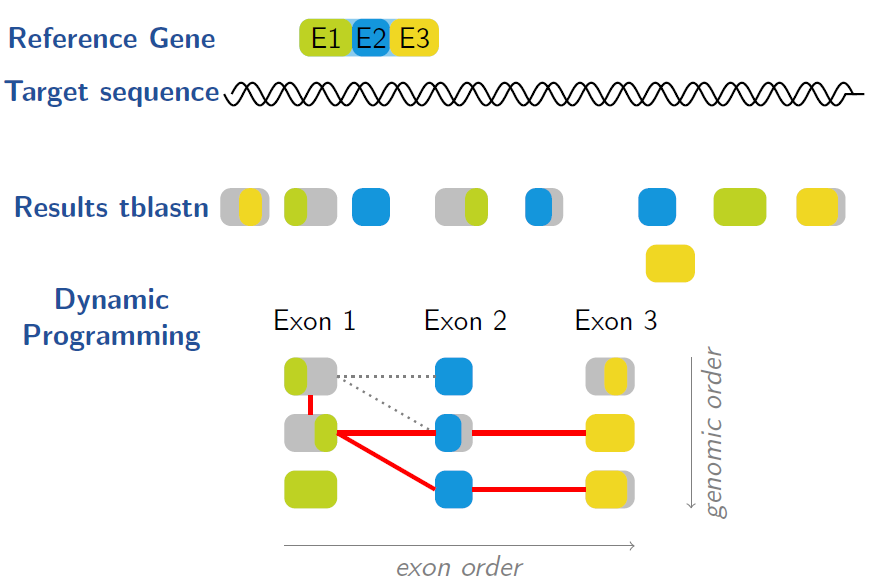
\includegraphics[width=\linewidth]{schema}
\caption{Illustration of the GeMoMa algorithm. GeMoMa uses \texttt{tblastn} to search for homologs of all (partially) coding exons of the reference transcript. Subsequently, a dynamic programming algorithm is used to determine the best combination of the hits.}
\end{figure}

\clearpage

\section{GeMoMa in a nutshell}

There are 7 steps that are divided into 3 phases. However, if you do not have any RNA-seq data you can skip the first phase.
This guide only provides a rough overview. If your are interested in individual parameters you can call:
\begin{verbatim}
java -jar GeMoMa-<version>.jar CLI <toolname>
\end{verbatim}
which will provide descriptions of all available parameters.

Note that homology-based gene prediction only infers genes with known counterparts in at least one reference organism. Therefore, homology-based gene prediction may miss genes for which counterparts are missing in the reference organisms, even if they are expressed and can be found in the RNA-seq data. On the other hand, homology-based gene prediction allows inference of genes that are not or rarely expressed in the RNA-seq samples.

\begin{figure}[h]
\includegraphics[width=\linewidth]{{drawing_pipeline5}.pdf}
\caption{GeMoMa workflow. Solid blue items represent input data sets, dashed blue items are optional inputs, green boxes represent GeMoMa modules, while grey boxes represent external modules. The GeMoMa Annotation Filter allows to combine predictions from different reference species. RNA-seq data is optional.}
\end{figure}

\clearpage

\subsection{Quick start}
We provide three scripts:
\begin{enumerate}
	\item A test script checking whether GeMoMa runs on your system on some tiny toy data: \texttt{tests.sh}. Example data can be found in directory \texttt{tests/gemoma/}.
	\item An application script allowing to start the complete GeMoMa workflow with minimal parameter input using the individual modules: \texttt{run.sh}. If you like to run the workflow with standard parameters and without any tricks for speed up you can just use this script.
\begin{itemize}
	\item Without RNA-seq data:
\begin{verbatim}
./run.sh <search> <target-genome> <ref-anno> <ref-genome>
         <out-dir>
\end{verbatim}	
	\item With RNA-seq data:
\begin{verbatim}
./run.sh <search> <target-genome> <ref-anno> <ref-genome>
         <out-dir> <lib-type> <mapped-reads>
\end{verbatim}
\end{itemize}
	\item An application script allowing to start the complete GeMoMa workflow with minimal parameter input using the GeMoMaPipeline module: \texttt{pipeline.sh}. If you like to run the workflow with standard parameters and without any tricks for speed up you can just use this script.
\begin{itemize}
	\item Without RNA-seq data:
\begin{verbatim}
./pipeline.sh <search> <target-genome> <ref-anno>
              <ref-genome> <threads> <out-dir>
\end{verbatim}	
	\item With RNA-seq data:
\begin{verbatim}
./pipeline.sh <search> <target-genome> <ref-anno>
              <ref-genome> <threads> <out-dir>
              <lib-type> <mapped-reads>
\end{verbatim}
\end{itemize}
\end{enumerate}
where
\begin{enumerate}
	\item \texttt{search} is a switch for the search algorithm to be used, either \texttt{tblastn} or \texttt{mmseqs}
	\item \texttt{target-genome} is the genome of the target organism (FastA)
	\item \texttt{ref-anno} is the annotation of the reference organism (GFF/GTF)
	\item \texttt{ref-genome} is the genome of the reference organism (FastA)
	\item \texttt{threads} the number of threads to be used
	\item \texttt{out-dir} is the output directory
	\item \texttt{lib-type} is the RNA-seq library type\\
		(\verb"{FR_UNSTRANDED, FR_FIRST_STRAND, FR_SECOND_STRAND}")
	\item \texttt{mapped-reads} are the mapped RNA-seq reads (SAM/BAM)
\end{enumerate}

\clearpage

\subsection{Phase 1: Preprocessing RNA-seq data}
For this phase, you need RNA-seq data and a reference sequence or assembly of your target organism.
This allows for inferring experimental verified introns and coverage. In the following command lines ''\verb"..."`` should be replaced by your specific parameters.

\begin{enumerate}
\item	Run your favorite read mapper (e.g. TopHat, \ldots) on your RNA-seq data
\item	Extract introns (and coverage) running: 
\begin{verbatim}
java -jar GeMoMa-<version>.jar CLI ERE ...
\end{verbatim}
\item	Optionally denoise the extracted introns running: 
\begin{verbatim}
java -jar GeMoMa-<version>.jar CLI DenoiseIntrons ...
\end{verbatim}
\end{enumerate}

\subsection{Phase 2: Prediction candidate transcripts}
For this phase, you need at least one reference organism with reference sequence/assembly and annotation as well as a reference sequence/assembly for the target organism.
Keep in mind that the outcome of GeMoMa highly depends on the quality of the reference annotation.
It is possible to run step 3 to 5 with multiple reference organisms.

\begin{enumerate}
\setcounter{enumi}{2}
\item Extract CDS-parts (and proteins) of the reference organism running:
	\begin{verbatim}
	java -jar GeMoMa-<version>.jar CLI Extractor ...
	\end{verbatim}
\item Find homologous parts in the target organism running: 
	\begin{verbatim}
	tblastn -outfmt "6 std sallseqid score nident positive gaps
	         ppos qframe sframe qseq sseq qlen slen salltitles" ...
	\end{verbatim}
	The output format of tblastn is essential for GeMoMa. Since version 1.6, we also allow to use mmseqs as search algorithm. Mmseqs is typically faster than tblastn. For more details we refer to the script \verb+run.sh+.
\item Find homologous candidate transcripts in the target organism running:
	\begin{verbatim}
	java -jar GeMoMa-<version>.jar CLI GeMoMa ...
	\end{verbatim}
	Since version 1.4, p=10 and ct=0.4 are new default values.
\end{enumerate}

\subsection{Phase 3: Aggregate and filter predictions}
For this phase, you need only the output of step 5.
If you ran the second phase for multiple reference organisms, the individual predictions can now be combined in this step.

\begin{enumerate}
\setcounter{enumi}{5}
\item Aggregate predictions running: 
	\begin{verbatim}
	java -jar GeMoMa-<version>.jar CLI GAF ...
	\end{verbatim}
\item Predict UTRs and rename predictions running: 
	\begin{verbatim}
	java -jar GeMoMa-<version>.jar CLI AnnotationFinalizer ...
	\end{verbatim}
\end{enumerate}

\clearpage
\section{Miscellaneous}

\subsection{Help section and parameter description}
If you like to receive more information about the available tools and parameters please enter
\begin{verbatim}
java -jar GeMoMa-<version>.jar CLI
\end{verbatim}
and follow the instructions.

\subsection{Check extracted introns}
If you like to check whether the extracted introns (cf. ERE) show the expected distribution of conserved di-nucleotides (cf. canonical splice sites), we have implemented the module CheckIntrons that can be used as follows:
\begin{verbatim}
java -jar GeMoMa-<version>.jar CLI CheckIntrons ...
\end{verbatim}

\subsection{Benchmarking}
Benchmarking is essential to compare different gene prediction approaches. If you use a target organism where the annotation is known, the prediction can be compared to this known annotation and performance measures like sensitivity and specificity can be computed. In case of a target organism without known gene annotation, BUSCO is often used to compare or measure the quality of the gene annotation. For both cases, we provide additional modules that help to analyze the gene prediction.

\subsubsection{Sensitivity and specificity}
Given some gold standard gene annotation, gene predictions can be compared in terms of sensitivity and specificity. There are several tools available that can do this, including the eval package  and gffcompare. However, they all have some problems, such as runtime or handling experimentally verified genes. For these reasons, we decided to implement our own benchmarking module called Analyzer that can be used as follows:
\begin{verbatim}
java -jar GeMoMa-<version>.jar CLI Analyzer ...
\end{verbatim}

In addition, this module allows retrieving a table with pairs of true and predicted annotations and F1 measure between these annotations. This table can be used for instance for analyzing the predicted annotation, plotting the F1 measure vs. sensitivity and comparing different annotations in detail. The R script analyze.r can be used for this purpose and is provided with the package.

\subsubsection{BUSCORecomputer}
If no gene annotation of the target organism is known, it is difficult to assess the quality of a predicted gene annotation. For this case, BUSCO has been proposed (\url{https://doi.org/10.1093/bioinformatics/btv351}), which is \textit{\textbf{B}enchmarking \textbf{U}niversal \textbf{S}ingle-\textbf{C}opy \textbf{O}rthologs}. BUSCO thus checks whether there is a single gene prediction for each universal ortholog of a taxon that should occur only once. However, alternative transcripts cause problems in BUSCO as they can increase the number of genes designated as \textit{duplicated}. For this reason, the BUSCO authors recommend using a single transcript per gene. Unfortunately, this is also subject to some caveats, as the selection of a single transcript per gene is not straightforward. Sometimes one transcript is accepted as ortholog and another transcript not. Therefore, one might underestimate the number of \textit{complete} genes.

For these reasons, we implemented a module called BUSCORecomputer, which uses the result of BUSCO and the gene-transcript relationship to recompute the percentage of complete and duplicated genes.
\begin{verbatim}
java -jar GeMoMa-<version>.jar CLI BUSCORecomputer ...
\end{verbatim}

\subsection{General speed-up}
If you
\begin{enumerate}
\item like to speed-up the computation and
\item have lots of compute cores,
\end{enumerate}
you might accelerate GeMoMa using the following tricks:

\subsubsection{RNA-seq data}
If you have a lot of RNA-seq samples you can map them independently. Afterwards, you can run ERE on each of the mapped read data sets (SAM/BAM). However, if you like to use the results of these runs in GeMoMa it is a bit annoying to set a lot of intron and coverage files as parameters. For this reason, we implemented two helper classes allowing to combine introns and coverage form independent runs:

\begin{verbatim}
java -cp GeMoMa-<version>.jar projects.gemoma.CombineIntronFiles
     <output name> <input0> <input1> ...
java -cp GeMoMa-<version>.jar projects.gemoma.CombineCoverageFiles
     <output name> <input0> <input1> ...
\end{verbatim}

Instead of listing all files, you can also use wildcards to easily combine individual coverage or intron files.

\subsubsection{Search and GeMoMa}
If you have large data sets, i.e., a large number of lines in the CDS-parts file, you can split the job in several independent jobs. Splitting the job can be done using
\begin{verbatim}
java -cp GeMoMa-<version>.jar projects.FastaSplitter <CDS-parts> 
     <numberOfSplits> "_"
\end{verbatim}

This will result in several independent FastA files containing some CDS-parts. You can run steps 4 and 5 on these individual parts.
Finally, you have to concatenate the resulting predicted annotations, protein, \ldots before starting step 6.

\subsection{GeMoMaPipeline}
If you only have a compute server and no compute cluster, the general speed-up described in the last section can directly be addressed without any manual interplay using the module GeMoMaPipeline. The module runs the complete pipeline as one job and allows to exploit the complete compute power of a server using multi-threading. 
However, this module can \textbf{only} exploit the compute power of a single server and does not distribute the partial jobs to a compute cluster.

If you like to receive more information about GeMoMaPipeline and its parameters please enter
\begin{verbatim}
java -jar GeMoMa-<version>.jar GeMoMaPipeline
\end{verbatim}
and follow the instructions.


\subsection{Runtime example}
To give an impression on the run of GeMoMaPipeline, we have run it with different number of threads and different search algorithms.
As example the annotation of \emph{A. thaliana} was predicted based on three reference organisms and RNA-seq data:
\begin{verbatim}
java -jar GeMoMa-1.7.jar GeMoMaPipeline threads=<threads> 
     tblastn=$tblastn b=$bpath m=$mpath GeMoMa.Score=ReAlign
     AnnotationFinalizer.r=NO o=true p=false t=TAIR10_chr_all.fas 
     s=own i=AL g=Arabidopsis_lyrata.v.1.0.31.dna.genome.fa
     a=Arabidopsis_lyrata.v.1.0.31.chr.gff3 
     s=own i=BO g=Boleraceacapitata_446_v1.0.fa
     a=Boleraceacapitata_446_v1.0.gene_exons.gff3
     s=own i=BS g=Bstricta_278_v1.fa
     a=Bstricta_278_v1.2.gene_exons.gff3
     r=MAPPED ERE.m=AlignedSorted-2pass.bam
\end{verbatim}
Runtime was measured with the Linux command \verb+time+.
The runtime issue for tblastn version 2.6.0 until 2.10.1 has been reported to NCBI (TRACKING:000412000006306). NCBI could reproduce the problem and will hopefully fix it soon.

\begin{table}[ht]\centering
\begin{tabular}{|r||r|r|r|}
\hline
threads	&tblastn 2.5.0+	&tblastn 2.10.1+	&mmseqs v11%\footnote{\verb+mmseqs version+ returns \verb+e1a1c1226ef22ac3d0da8e8f71adb8fd2388a249+}}
\\
\hline\hline
1	&34:54:45	&NA	&07:38:36\\\hline
4	&09:14:19	&NA	&02:22:39\\\hline
16	&02:41:48	&63:13:09	&00:48:32\\\hline
64	&00:58:23	&18:53:00	&00:29:00\\\hline
\end{tabular}
\caption{
Runtime comparison of the GeMoMaPipeline. The runtime is given using the format hh:mm:ss.
%compute node specificcation
The prediction accuracy was identical for the different blast versions and very similar for mmseqs.
}
\end{table}

Of course, the runtime also depends on the hardware, the reference organisms and the size of the target genome.


\subsection{Genome-wide vs. specific genes}
By default, GeMoMa tries to make predictions for all CDS of the reference organism in the target organism. Hence, we call this a genome-wide approach. Additionally, Extractor and GeMoMa have an option for filtering based on a list of some reference CDS (cf. parameter \texttt{selected}). This approach allows to further speed up the predictions especially if one is interested only in a certain part of the annotation.

\subsection{Add attributes}
Sometimes it might be beneficial to add attributes to the structural annotation, e.g., you could predict functional annotation with InterProScan and might use them in GAF or display them in genome browsers like IGV or WebApollo. Hence, GeMoMa provides an additional module called AddAttribute which allows to add attributes to a structural annotation using an additional table.

\begin{verbatim}
java -jar GeMoMa-<version>.jar CLI AddAttribute ...
\end{verbatim}

\subsection{Synteny}
Comparing different genome assemblies or organisms, synteny is sometimes of interest. There are specialized programs that compute synteny by comparing chromosomes or contigs of different species. These programs need to do some kind of alignment or mapping. As GeMoMa computes alignments of proteins from a reference organism to a target organism, these gene predictions can be used to infer synteny on a gene level with almost no additional runtime. Since version 1.7, GeMoMa includes a module called SyntenyChecker and an R script (see below).

\begin{verbatim}
java -jar GeMoMa-<version>.jar CLI SyntenyChecker ...
\end{verbatim}

The result of SyntenyChecker can be visualized using the R script synplot.r. An example how to use both, SyntenyChecker and synplot.r is given at the end of run.sh. However, as the toy data is too small for synteny computation, it is only given in the comments.

\subsection{Galaxy integration}
GeMoMa provides a command line interface as well as everything to be integrated in your local Galaxy instance. For creating the XML files that are needed for integration into Galaxy, just run: 
\begin{verbatim}
createGalaxyIntegration.sh <version>
\end{verbatim}

Alternatively, you can run the individual commands on your own using the command line
\begin{verbatim}
java -jar GeMoMa-<version>.jar --create
\end{verbatim}
If you like to modify some VM arguments for the java calls made by Galaxy you can alter them for each sub-tool individually. If you like to allow GeMoMa to allocate at most 40GB of RAM, you may do so by running
\begin{verbatim}
java -jar GeMoMa-<version>.jar --create GeMoMa -Xmx40g
\end{verbatim}
to create the corresponding XML integration for GeMoMa.

\myPortrait{landscape}
\section{Real example}
In this section, we show how to run the main modules and analysis with GeMoMa using some real data from NCBI (\emph{Arabidopsis thaliana} and \emph{Arabidopsis lyrata}). You can rerun this example using the script \verb+real-example.sh+. First of all, we need some data:

\begin{Verbatim}
mkdir NCBI
cd NCBI
wget -c https://ftp.ncbi.nlm.nih.gov/genomes/all/GCF/000/001/735/GCF_000001735.4_TAIR10.1/GCF_000001735.4_TAIR10.1_genomic.fna.gz
wget -c https://ftp.ncbi.nlm.nih.gov/genomes/all/GCF/000/001/735/GCF_000001735.4_TAIR10.1/GCF_000001735.4_TAIR10.1_genomic.gff.gz
wget -c https://ftp.ncbi.nlm.nih.gov/genomes/all/GCF/000/004/255/GCF_000004255.2_v.1.0/GCF_000004255.2_v.1.0_genomic.fna.gz
wget -c https://ftp.ncbi.nlm.nih.gov/genomes/all/GCF/000/004/255/GCF_000004255.2_v.1.0/GCF_000004255.2_v.1.0_genomic.gff.gz
cd ..
\end{Verbatim}

\subsection{GeMoMaPipeline}
We try to predict genes in \emph{Arabidopsis lyrata} based on the gene annotation of a single reference organism, here \emph{Arabidopsis thaliana}. We do not like to rename the predictions (\verb+AnnotationFinalizer.r=NO+) or obtain the predicted proteins (\verb+p=false+). However, we like to have the individual predictions of GeMoMa for each reference species (\verb+o=true+). This allows to rerun the GAF with slightly different parameter settings, obtaining new results very quickly without the need of time-consuming search and GeMoMa steps.

GeMoMaPipeline with default parameters and without RNA-seq evidence predicts a single transcript per gene. As we like to demonstrate the utility of BUSCORecomputer later, we modify the parameter \verb+GAF.a+ to allow multiple transcript predictions per gene:

\begin{Verbatim}
java -jar GeMoMa-1.8.jar CLI GeMoMaPipeline threads=20 AnnotationFinalizer.r=NO p=false o=true 
	t=NCBI/GCF_000004255.2_v.1.0_genomic.fna.gz GAF.a="pAA>=0.7" outdir=output/
	i=thaliana a=NCBI/GCF_000001735.4_TAIR10.1_genomic.gff.gz g=NCBI/GCF_000001735.4_TAIR10.1_genomic.fna.gz 
\end{Verbatim}

\subsubsection{Tips}
Depending on your default settings and the amount of data, you might have to increase the memory that can be used by setting the VM arguments for initial and maximal heap size, e.g., \verb+-Xms200G -Xmx400G+.\\

GeMoMaPipeline writes its version and all parameters that are no files at the beginning of the predicted annotation. This allows to check parameters at any time point.\\

If GeMoMaPipline crashes with an Exception, the parameter \verb+restart+ can be used to restart the latest GeMoMaPipeline run, which was finished without results, with very similar parameters. This allows to avoid time-consuming steps like the search that were successful in the latest GeMoMaPipeline run.\\

If you like to use several reference organisms, you can use the parameters \verb+a+ and \verb+g+ several times, but you new to add the parameter \verb+s+. Additionally, we recommend to use the parameter \verb+i+, which allows providing an ID for each reference organism:
\begin{Verbatim}
java -jar GeMoMa-1.8.jar CLI GeMoMaPipeline threads=20 AnnotationFinalizer.r=NO p=false o=true 
	t=NCBI/GCF_000004255.2_v.1.0_genomic.fna.gz outdir=output/
	s=own i=<speciesA> a=<speciesA.gff> g=<speciesA.fna>
	s=own i=<speciesB> a=<speciesB.gff> g=<speciesC.fna>
	s=own i=<speciesC> a=<speciesC.gff> g=<speciesC.fna>
\end{Verbatim}
If you like to use mapped RNA-seq data, you have to use the parameters \verb+r+ and \verb+ERE.m+:
\begin{Verbatim}
java -jar GeMoMa-1.8.jar CLI GeMoMaPipeline threads=20 AnnotationFinalizer.r=NO p=false o=true
	t=NCBI/GCF_000004255.2_v.1.0_genomic.fna.gz outdir=output/ r=MAPPED ERE.m=<SAM/BAM>
	a=NCBI/GCF_000001735.4_TAIR10.1_genomic.gff.gz g=NCBI/GCF_000001735.4_TAIR10.1_genomic.fna.gz 
\end{Verbatim}
If you have multiple mapped RNA-seq data sets, for example 3, you can use them all
\begin{Verbatim}
java -jar GeMoMa-1.8.jar CLI GeMoMaPipeline threads=20 AnnotationFinalizer.r=NO p=false o=true 
	t=NCBI/GCF_000004255.2_v.1.0_genomic.fna.gz outdir=output/ r=MAPPED ERE.m=<SAM/BAM1> ERE.m=<SAM/BAM2> ERE.m=<SAM/BAM3>
	a=NCBI/GCF_000001735.4_TAIR10.1_genomic.gff.gz g=NCBI/GCF_000001735.4_TAIR10.1_genomic.fna.gz 
\end{Verbatim}
If you like to use predict only homologs for a specific gene, gene family or set of genes from the reference organism, you can use the parameter \verb++. You have to provide a list of reference transcript ID as a file and pass it to the parameter:
\begin{Verbatim}
java -jar GeMoMa-1.8.jar CLI GeMoMaPipeline threads=20 AnnotationFinalizer.r=NO p=false o=true 
	t=NCBI/GCF_000004255.2_v.1.0_genomic.fna.gz outdir=output/ selected=<SELECTED>
	a=NCBI/GCF_000001735.4_TAIR10.1_genomic.gff.gz g=NCBI/GCF_000001735.4_TAIR10.1_genomic.fna.gz 
\end{Verbatim}
If you like to rename your predictions, you can use the parameters \verb+AnnotationFinalizer.r+. This parameter has three options
\begin{itemize}
\item \verb+NO+, which does not rename the transcripts,
\item \verb+SIMPLE+, which renames the predictions according to the schema \verb+<PREFIX><digit>+, and
\item \verb+COMPOSED+, which renames the predictions according to the schema \verb+<PREFIX><contig_identifier><INFIX><digit><SUFFIX>+ (cf. TAIR name schema)
\end{itemize}
where upper case place holders (such as \verb+<PREFIX>+) are determined by the user via additional parameters and lower case place holders are determined internally. Hence, additional parameters need to be set for the options \verb+SIMPLE+ and \verb+COMPOSED+, e.g., the prefix via \verb+AnnotationFinalizer.p+. Furthermore, you can decide whether the name should be used for an additional GFF attribute \verb+name+ or for the existing GFF attribute \verb+ID+ and \verb+parent+. You can choose between these to options using the parameter \verb+AnnotationFinalizer.n+. 
\begin{Verbatim}
java -jar GeMoMa-1.8.jar CLI GeMoMaPipeline threads=20 AnnotationFinalizer.r=SIMPLE AnnotationFinalizer.p=<PREFIX>
	t=NCBI/GCF_000004255.2_v.1.0_genomic.fna.gz outdir=output/ o=true
	a=NCBI/GCF_000001735.4_TAIR10.1_genomic.gff.gz g=NCBI/GCF_000001735.4_TAIR10.1_genomic.fna.gz 
\end{Verbatim}
If you like to retrieve the predictions as proteins, CDS, or genomic regions, you can use the parameters \verb+p+, \verb+pc+, and \verb+pgr+, respectively. Internally, GeMoMaPipeline will call Extractor on the final prediction to obtain the desired files. Alternatively, you can run Extractor on you own. 
\begin{Verbatim}
java -jar GeMoMa-1.8.jar CLI GeMoMaPipeline threads=20 AnnotationFinalizer.r=NO o=true 
	t=NCBI/GCF_000004255.2_v.1.0_genomic.fna.gz outdir=output/ p=true pc=true pgr=true
	a=NCBI/GCF_000001735.4_TAIR10.1_genomic.gff.gz g=NCBI/GCF_000001735.4_TAIR10.1_genomic.fna.gz 
\end{Verbatim}
If you like to use protein input as reference, you can also use GeMoMa, although it is not able to utilize intron position conservation in this case. Given a \verb+ref-protein.fasta+, you can run GeMoMaPipeline:
\begin{Verbatim}
java -jar GeMoMa-1.8.jar CLI GeMoMaPipeline threads=20 AnnotationFinalizer.r=NO p=false o=true 
	t=NCBI/GCF_000004255.2_v.1.0_genomic.fna.gz outdir=output/
	s=pre-extracted c=ref-proteins.fasta
\end{Verbatim}
If you like to combine GeMoMa predictions with given external annotation \verb+external.gff+, e.g., from \emph{ab-initio} gene prediction, you can use the parameter \verb+e+:. In this case we highly recommend to use the optional parameters \verb+i+ and verb+ID+ to be able to clearly distinguish the origin of a prediction in the final annotation:
\begin{Verbatim}
java -jar GeMoMa-1.8.jar CLI GeMoMaPipeline threads=20 AnnotationFinalizer.r=NO o=true 
	t=NCBI/GCF_000004255.2_v.1.0_genomic.fna.gz outdir=output/ p=true pc=true pgr=true
	i=<REFERENCE_ID> a=NCBI/GCF_000001735.4_TAIR10.1_genomic.gff.gz g=NCBI/GCF_000001735.4_TAIR10.1_genomic.fna.gz 
	ID=<EXTERNAL_ID> e=external.gff
\end{Verbatim}
\clearpage
\subsection{Synteny}
If you like to compare the order of genes between two organisms the module SyntenyChecker that is run by default at the end of the pipeline can be used. This module creates a table that can be visualized with the R script \verb+synplot.r+:
\begin{verbatim}
Rscript synplot.r output/reference_gene_table.tabular 5 output/test lyrata
\end{verbatim}
\vspace{-5mm}
\begin{center}\includegraphics[width=0.3\linewidth]{{test-synteny-k=5}.pdf}\end{center}

\subsection{Analyzer}
Based on the results of the previous subsection and the gene annotation from NCBI, we run the Analyzer to evaluate sensitivity and specificity:
\begin{Verbatim}
java -jar GeMoMa-1.8.jar CLI Analyzer t=NCBI/GCF_000004255.2_v.1.0_genomic.gff.gz
	n="test" p=output/final_annotation.gff w=YES outdir=output/
\end{Verbatim}

Using the parameter \verb+w=YES+, the Analyzer writes a table analyzed in detail. Some interesting aspects can be visualized using the R script \verb+analyze.r+ that is include in GeMoMa:
\begin{verbatim}
Rscript analyze.r output/Comparison_0.tabular
\end{verbatim}

This script produces several outputs that allow to judge the gene prediction, e.g.,\\
\includegraphics[width=0.3\linewidth,page=2]{{Comparison_0.tabular-comparison-with-truth}.pdf}
\includegraphics[width=0.3\linewidth,page=3]{{Comparison_0.tabular-comparison-with-truth}.pdf}
\includegraphics[width=0.3\linewidth,page=6]{{Comparison_0.tabular-comparison-with-truth}.pdf}

\subsubsection{Tips}
If you like to compare several gene predictions, e.g., several gene prediction programs or different parameter setting you can run the R script with several inputs. This will create a combined plot of F1 versus sensitivity:
\begin{verbatim}
Rscript analyze.r <name1=table1> <name2=table2> <name3=table3>
\end{verbatim}

\subsection{BuscoRecomputer}
Based on the results of the GeMoMaPipeline section, we like to evaluate the BUSCO score. First we extract all predicted proteins. This could be either done in the GeMoMaPipeline or explicitly via the module Extractor. As we need the assignment file for BUSCORecomputer, we use the Extractor as follows:
\begin{Verbatim}
java -jar GeMoMa-1.8.jar CLI Extractor Ambiguity=AMBIGUOUS p=true outdir=output/
	g=NCBI/GCF_000004255.2_v.1.0_genomic.fna.gz a=output/final_annotation.gff
\end{Verbatim}
Now, we can run BUSCO (which needs to be installed) on these proteins:
\begin{verbatim}
busco -i output/proteins.fasta -l embryophyta_odb10 -o busco -m proteins
\end{verbatim}
Finally, we can run BUSCORecomputer based on the BUSCO results and the assignment file:
\begin{verbatim}
java -jar GeMoMa-1.8.jar CLI BUSCORecomputer b=busco/full_table.tsv i=output/assignment.tabular outdir=output/
\end{verbatim}
Comparing the results, we clearly see that BUSCORecomputer lead to less \emph{duplicated} genes which is more realistic since the difference is explained by alternative transcripts and not different genes.  
If you have multiple transcripts per gene BUSCO has problems with the number of duplicated genes.
\begin{center}\begin{tabular}{ll}
BUSCO	&C:99.2\%[S:68.3\%,D:30.9\%],F:0.2\%,M:0.6\%,n:1614\\
BUSCORecomputer	&C:99.3\%[S:97.4\%,D:1.9\%],F:0.2\%,M:0.6\%,n:1614
\end{tabular}\end{center}
Slight differences in the percentages of complete (C), fragmented (F) or missing (M) BUSCOs might occur due to different rounding modes.


\myPortrait{portrait}
\section{Reference, questions and comments}
If you use GeMoMa please cite:\\[\medskipamount]
\emph{Using intron position conservation for homology-based gene prediction.}\\
J. Keilwagen, M. Wenk, J. L. Erickson, M. H. Schattat, J. Grau, and F. Hartung.\\
Nucleic Acids Research, 2016. doi: \href{https://doi.org/10.1093/nar/gkw092}{10.1093/nar/gkw092}\\[\medskipamount]
\emph{Combining RNA-seq data and homology-based gene prediction for plants, animals and fungi.}\\
J. Keilwagen, F. Hartung, M. Paulini, S. O. Twardziok, and J. Grau.\\
BMC Bioinformatics, 2018. doi: \href{https://doi.org/10.1186/s12859-018-2203-5}{10.1186/s12859-018-2203-5}\\
~\\
The complete documentation can be found at:\\
\url{http://www.jstacs.de/index.php/GeMoMa-Docs}\\
~\\
FAQs, release notes, \ldots can be found on the homepage:\\
\url{http://www.jstacs.de/index.php/GeMoMa}\\
~\\
Issues can be checked and reported at:\\
\url{https://github.com/Jstacs/Jstacs/issues?q=label\%3AGeMoMa}\\

~\\
For further questions or comments, please contact:\\
\href{mailto:jens.keilwagen@julius-kuehn.de?subject=GeMoMa manual}{jens.keilwagen@julius-kuehn.de}
\end{document}